
\chapter{Projekt i implementacja aplikacji internetowej w technologii Vue.js}
\section{Narzędzia i techonologie}
\subsection{Node.js}
Node.js jest środowiskiem uruchomieniowym umożliwiającym używanie języka Javascript poza przeglądarką. Środowisko to charakteryzuje asynchroniczność oraz sterowanie zdarzeniami. Asynchroniczność umożliwia wykonywanie wielu czynności w tym samym czasie bez względu na jednowątkowość wynikającą z ograniczenia języka Javascript. Sterowanie zdarzeniami jest rozwiązaniem typowym dla interfejsów graficznych. Zapewnia ono elastyczność oraz możliwość tworzenia bardziej interaktywnych elementów GUI. Ponadto Node.js udostępnia menenadżer pakietów środowiska Node (NPM - Node Package Manager) dający możliwość zarządzania zainstalowanymi funkcjonalnościami w prosty i przejrzysty sposób.
\subsection{Vue.js}
Vue.js to framework języka Javascript slużący do budowania interfejsów użytkownika. W stosunku do dwóch najpopularnieszych alternatyw - frameworków React oraz Angular - wyróżnia się prostotą, szybkością działania oraz niewielkim rozmiarem. Framework Vue.js został zaprojektowany tak, aby zapewnić jak największą elastyczność. Przy jego użyciu możliwe jest tworzenie nie tylko prostych komponentów, ale i aplikacji typu single-page-application oraz multi-page-application. 

Cechą charakterystyczną Vue.js jest wykorzystanie szablonów jako sposobu na powiązanie języka znaczników HTML z wartwą logiki Javascript. Powiązanie to umożliwia wykorzystywanie w prosty sposób instrukcji warunkowych oraz pętli do wyświetlanie zawartości aplikacji.   

\subsection{Vuex}
Vuex to biblioteka oferująca zcentralizowany magazyn danych dostępny dla wszystkich komponentów w aplikacji. Stan danych w magazynie Vuex jest zmieniany poprzez mutacje wykonywane w reakcji na działanie dyspozytora~\ref{rys:vuex}. Takie podejście, że dane z części backendowej aplikacji mogą zostać pobrane tylko raz, a później bedą one dostępne bezpośrednio w częsci frontendowej za pośrednictwem magazynu.

\begin{figure}[t]
\centering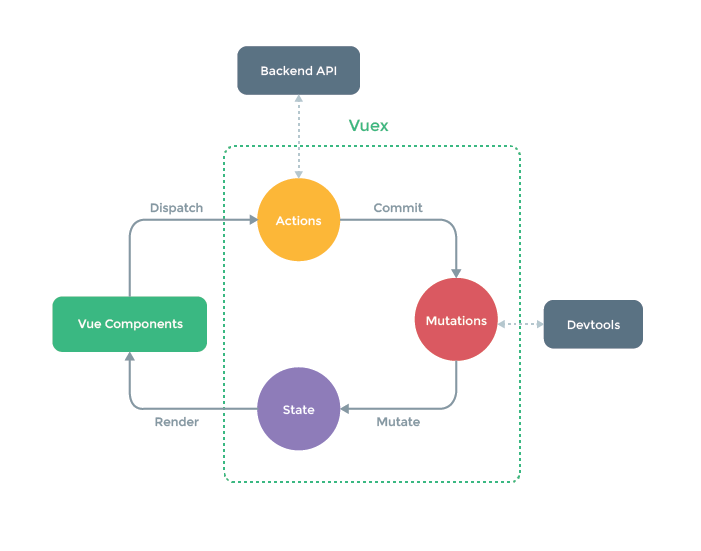
\includegraphics[width=\textwidth]{figures/vuex}
\caption{Schemat przepływu danych w Vuex.}\label{rys:vuex}
\end{figure}

\subsection{Jest}
W projekcie wykorzystano framework testowy Jest bedący częscią Vue Test Utils. Vue Test Utils to zestaw funkcjonalności upraszczających testowanie komponentów Vue.js. Zestaw ten zapewnia metody umożliwiające symulowanie działań użytkownika w aplikacji oraz przechwytywanie i porównywanie rezultatów tych interakcji z oczekiwanymi. Jest cechuje brak konieczności konfiguracji, izolacja testów oraz szybkość i bezpieczeństwo działania.
\subsection{Json Web Tokens}
Json Web Token jest otwartym standardem przesyłania zabezpieczonych danych. Dane w formacie Json są podpisywane cyfrowo co umożliwia weryfikacje uprawnień. W aplikacjach internetowych JWT stosowane są głownie do autoryzacji użytkowników oraz zapewnienia bezpieczeństwa przesyłanie informacji pomiędzy frotendem, a backendem. Niewielki rozmiar tokenu sprawia iż możliwe jest przesyłanie go w tre ści zapytania HTTP lub nawet w jego nagłówku. Ta cecha sprawia również, że token może być przechowywany w pamięci przeglądarki, eliminując konieczność ponownego uwierzytelniania po rozpoczęciu nowej sesji.
\subsection{Postman}
Postman jest zestawem narzędzi do testowania API (application programming interface). Zapewnia on możliwość wysyłania zapytań HTTP dowolnego typu oraz podgląd odpowiedzi i kodów błędów, jeśli takie wystąpiły. Główną zaletą Postmana jest możliwość tworzenia kolekcji zapytań, które ułatwiają organizację pracy podczas planowania połączeń pomiędzy częścią frontendową i backendową aplikacji. Dodatkowo narzędzie pozwala na wpółdzielenie kolekcji z zaproszonymi użytkownikami, co znacząco upraszcza proces testowania manualnego. Poza testowaniem manualnym Postman umożliwia tworzenie automatycznych testów przy pomocy języka Javascript. Dzięki generatorowi losowych danych możliwa jest symulacja działań nawet kilku tysięcy różnych użytkowników w systemie.
\subsection{Visual Studio Code}
Visual Studio Code jest edytorem kodu, którego głównymi zaletami jest wsparcie dla debugowania, inteligentnego uzupełniania kodu, refaktoryzacji oraz kontroli wersji. Dużą korzyścią płynącą z korzystania z program Visual Studio Code jest dostęp do rozszerzeń, usprawniających pracę z kodem w dowolnym języku programowania. Rozszerzenia zapewniają róznież wsparcie dla frameworków, w tym Vue.js, najbardziej istotnym dla tej części projektu. Mały rozmiar oraz wysoka wydajność znacznie przyśpieszają korzystanie z aplikacji i sprzyjają intensywnej iteracji rozwiązań.
\subsection{Axios}
Axios jest biblioteką języka Javascript służacą do wykonywania zapytań HTTP z poziomu Node.js lub przeglądarki. W aplikacjach internetowych wykorzystywany jest do uzyskiwania danych z części backendowej aplikacji. Axios bazuje na obietnicach (promise), co pozwala na obsługiwanie akcji asynchronicznie. Biblioteka może być użyta poprzez zwykły Javascript lub framework taki jak Vue.js. W porównaniu z innymi bibliotekami służacymi do wykonywania zapytań HTTP Axios oferuje wspracie dla starszych przeglądarek, możliwość ustawienia ograniczenia czasowego dla zapytań, ochronę przed CSRF (Cross-Site Request Forgery), a także automatyczną transformację danych JSON.
\subsection{Bootstrap}
\section{Widoki}
\subsection{Strona główna}
Strona główna aplikacji została stworzona na bazie szablonu Bootstrap o nazwie One Page Wonder(źródło). Zawiera ona krótki opis aplikacji, a także korzyści płynących z wykorzystania jej dla planistów, nauczycieli oraz uczniów. Pasek menu znajdujący się zawsze na górze strony jest stałym elementem aplikacji pojawiającym się w każdym z widoków. Pozwala on na przejście do widoków logowania i rejestracji, a przypadku gdy użytkownik jest już zalogowany na wylogowanie lub przejście do widoku szkoły. 
\begin{figure}[t]
\centering
\includegraphics[width=\textwidth]{figures/main}
\caption{Aplikacja internetowa - Strona głowna}\label{rys:main}
\end{figure}
\subsection{Widok szkoły}
Widok szkoły pozwala na przejście do dodawania danych potrzebnych do wygenerowania planu, a przypaku gdy plan został już wygenerowany jest również miejscem w którym jest on wyświetlany. Rozkład zajęć jest możliwy do wyświetlenia na trzy sposoby - z podziałem na klasy, nauczycieli lub sale lekcyjne.
\begin{figure}[t]
\centering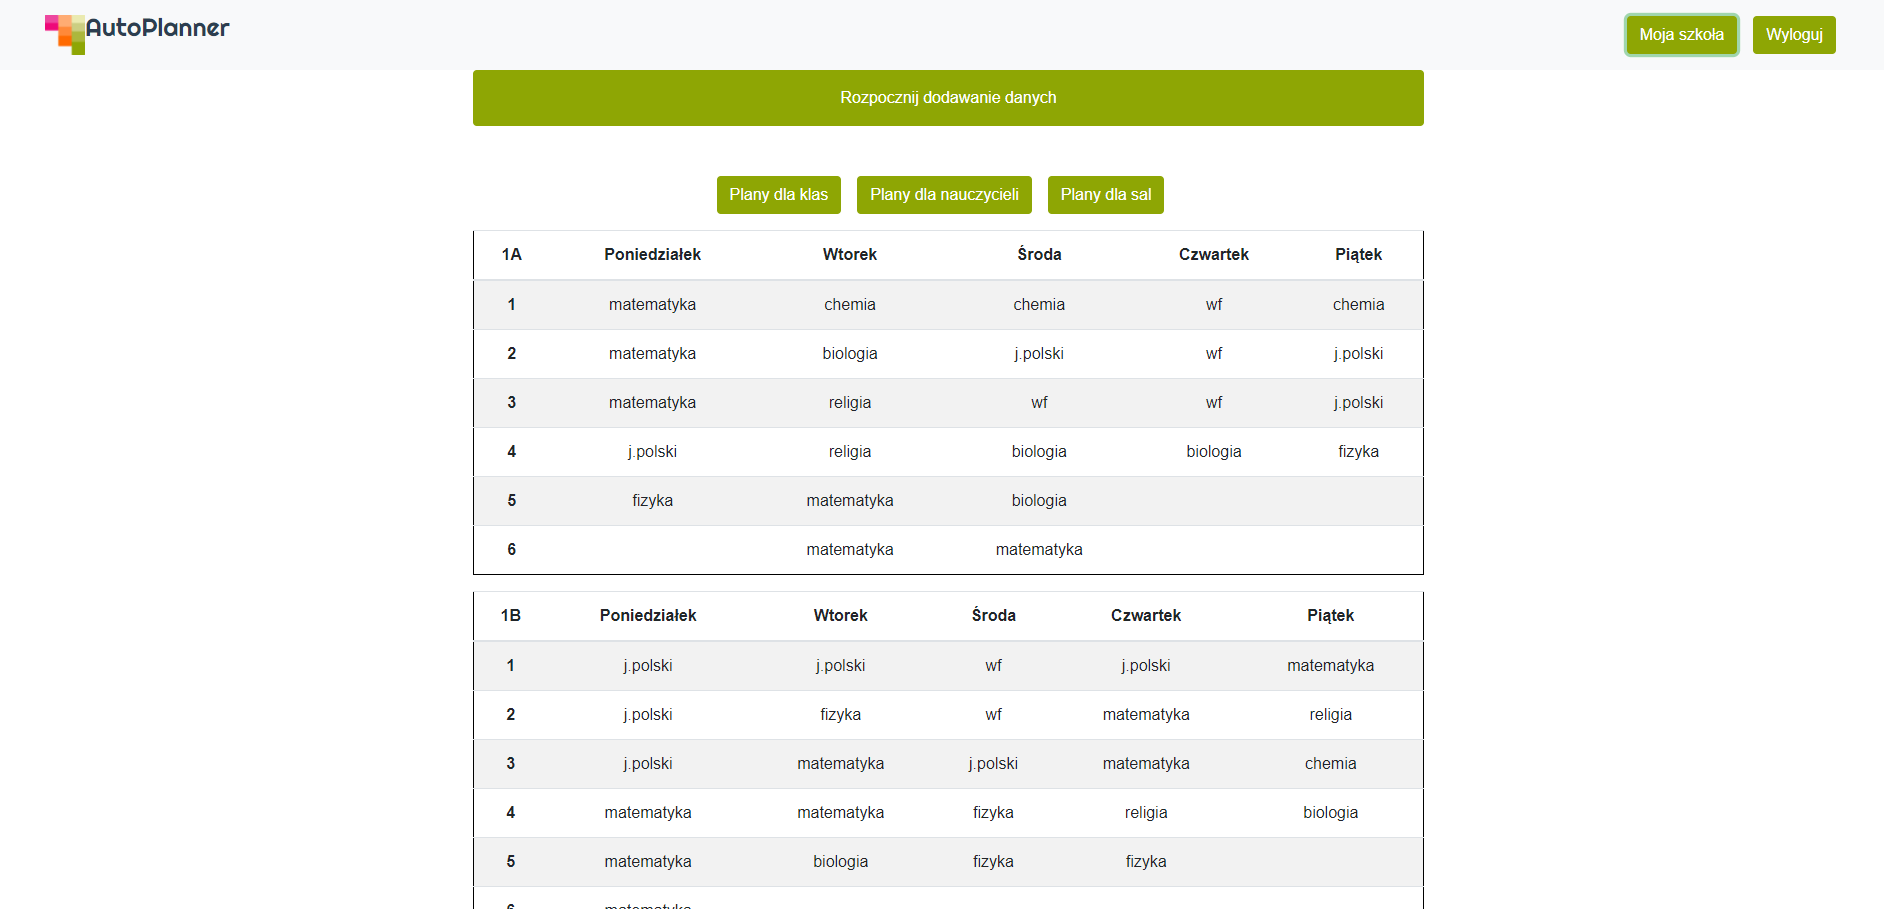
\includegraphics[width=\textwidth]{figures/school}
\caption{Aplikacja internetowa - Widok szkoły}\label{rys:school}
\end{figure}
\subsection{Rejestracja}
Widok rejestracji umożliwia utworzenie konta w serwisie. Od użytkownika wymaga się podania adresu email, nazwy użytkownika oraz hasła. Adres email musi być unikatowy. Wynika to z konieczności weryfikacji konta poprzez wiadomość wysłaną przy pomocy serwera SMTP. Rozwiązanie to ma na celu zapobieganie atakom na stronę poprzez masowe tworzenie nowych kont. 
\begin{figure}[t]
\centering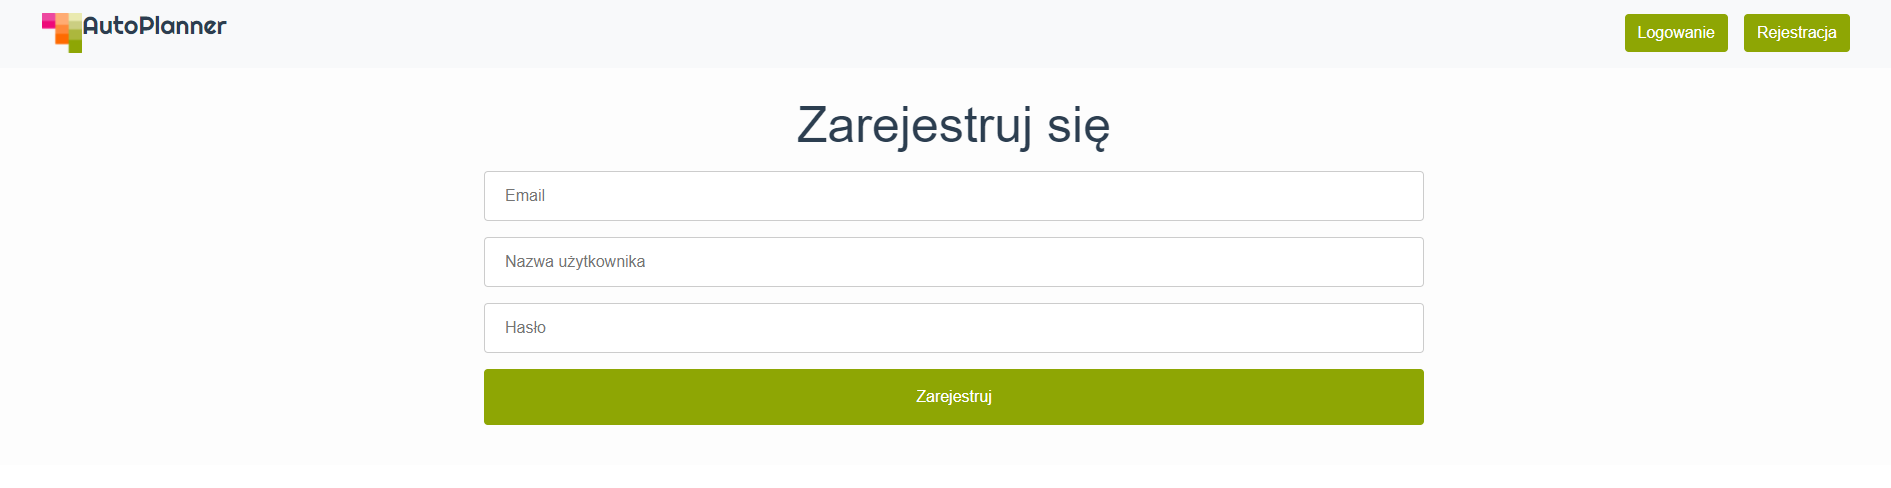
\includegraphics[width=\textwidth]{figures/register}
\caption{Aplikacja internetowa - Widok rejestracji}\label{rys:register}
\end{figure}
\subsection{Logowanie}
Widok logowania pozwala na dostęp do konta i zapisanych na nim danych z dowolnego urządzenia. Do uwierzytelnienia użytkownika wykorzystywany jest adres email oraz hasło podane w procesie rejestracji. Powodzenie procesu logowania powoduje otrzymanie przez aplikację tokenu JWT, zapisywanego w pamięci przeglądarki. W przypadku utraty hasła użytkownik posiada możliwość odzyskania go po podaniu adresu email powiązanego z istniejącym kontem.
\begin{figure}[t]
\centering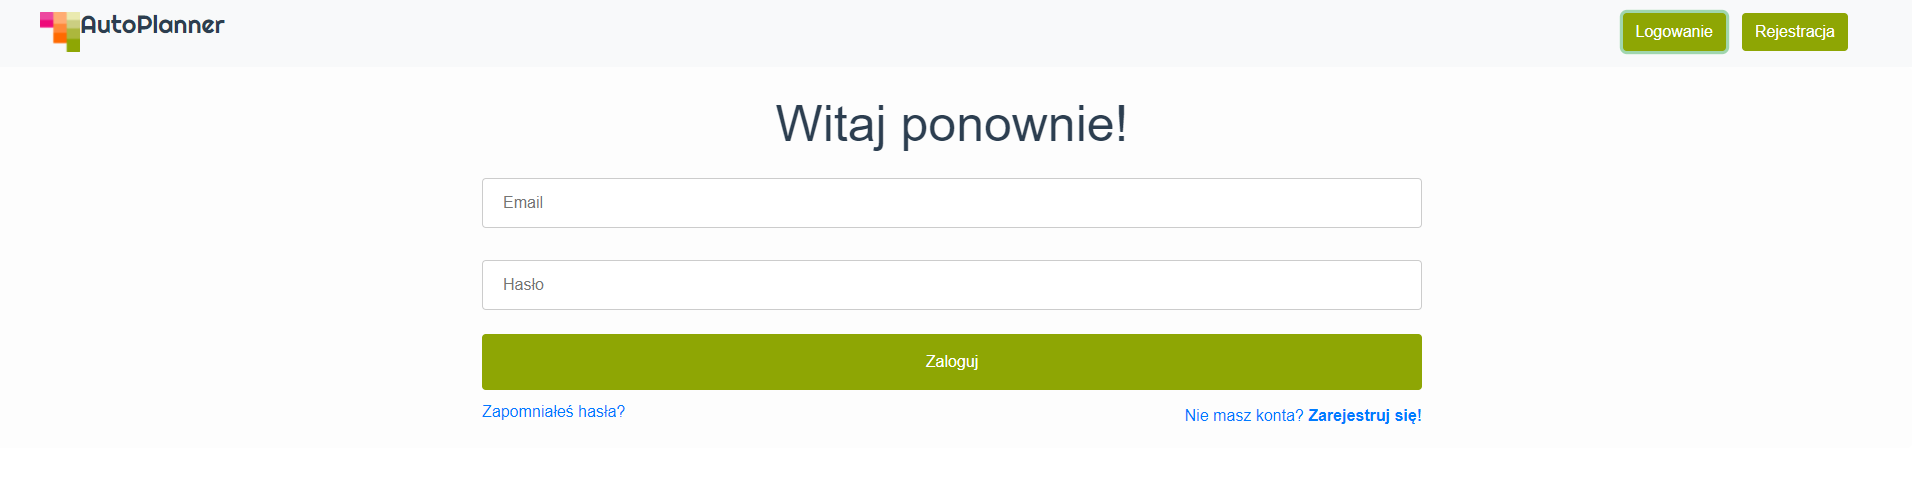
\includegraphics[width=\textwidth]{figures/login}
\caption{Aplikacja internetowa - Widok logowania}\label{rys:login}
\end{figure}

\subsection{Ankieta}
\begin{figure}[t]
\centering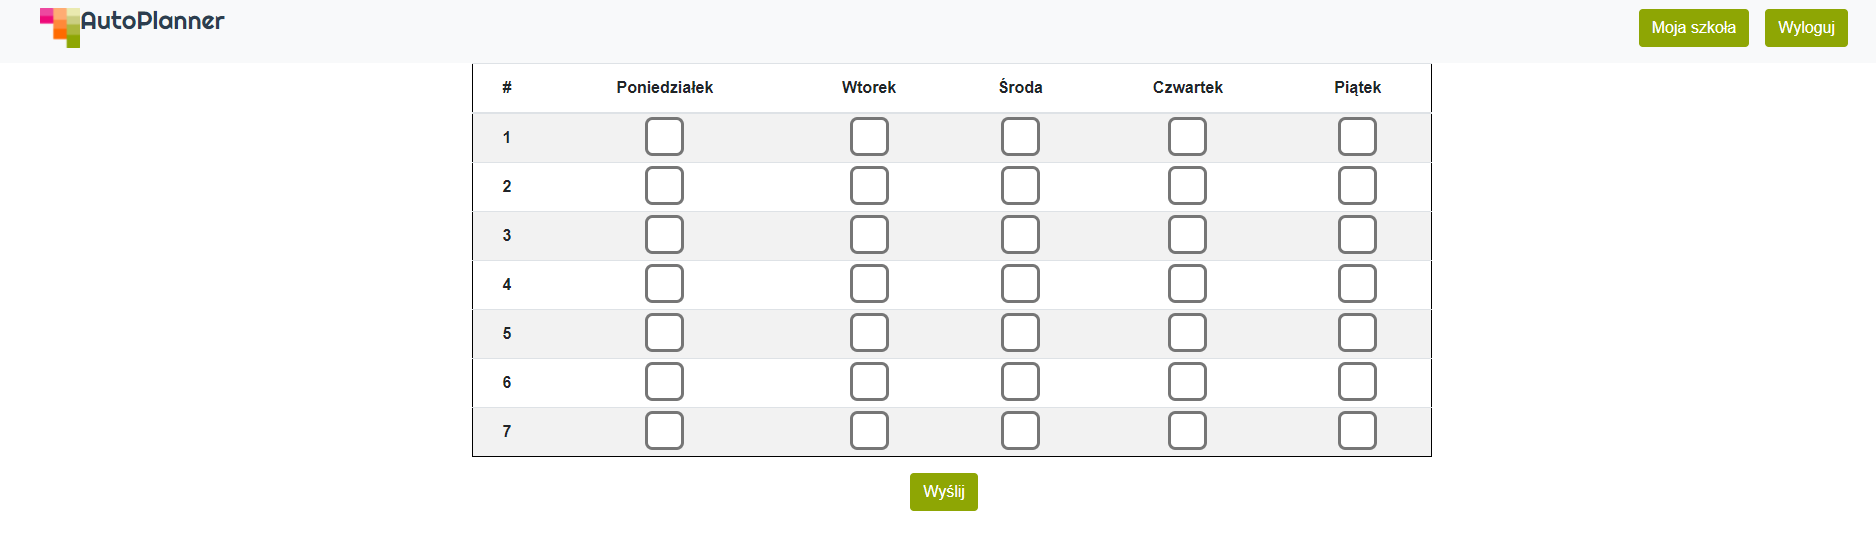
\includegraphics[width=\textwidth]{figures/poll}
\caption{Aplikacja internetowa - Widok ankiet dla nauczycieli}\label{rys:poll}
\end{figure}
\subsection{Dodawanie przedmiotów}
\begin{figure}[t]
\centering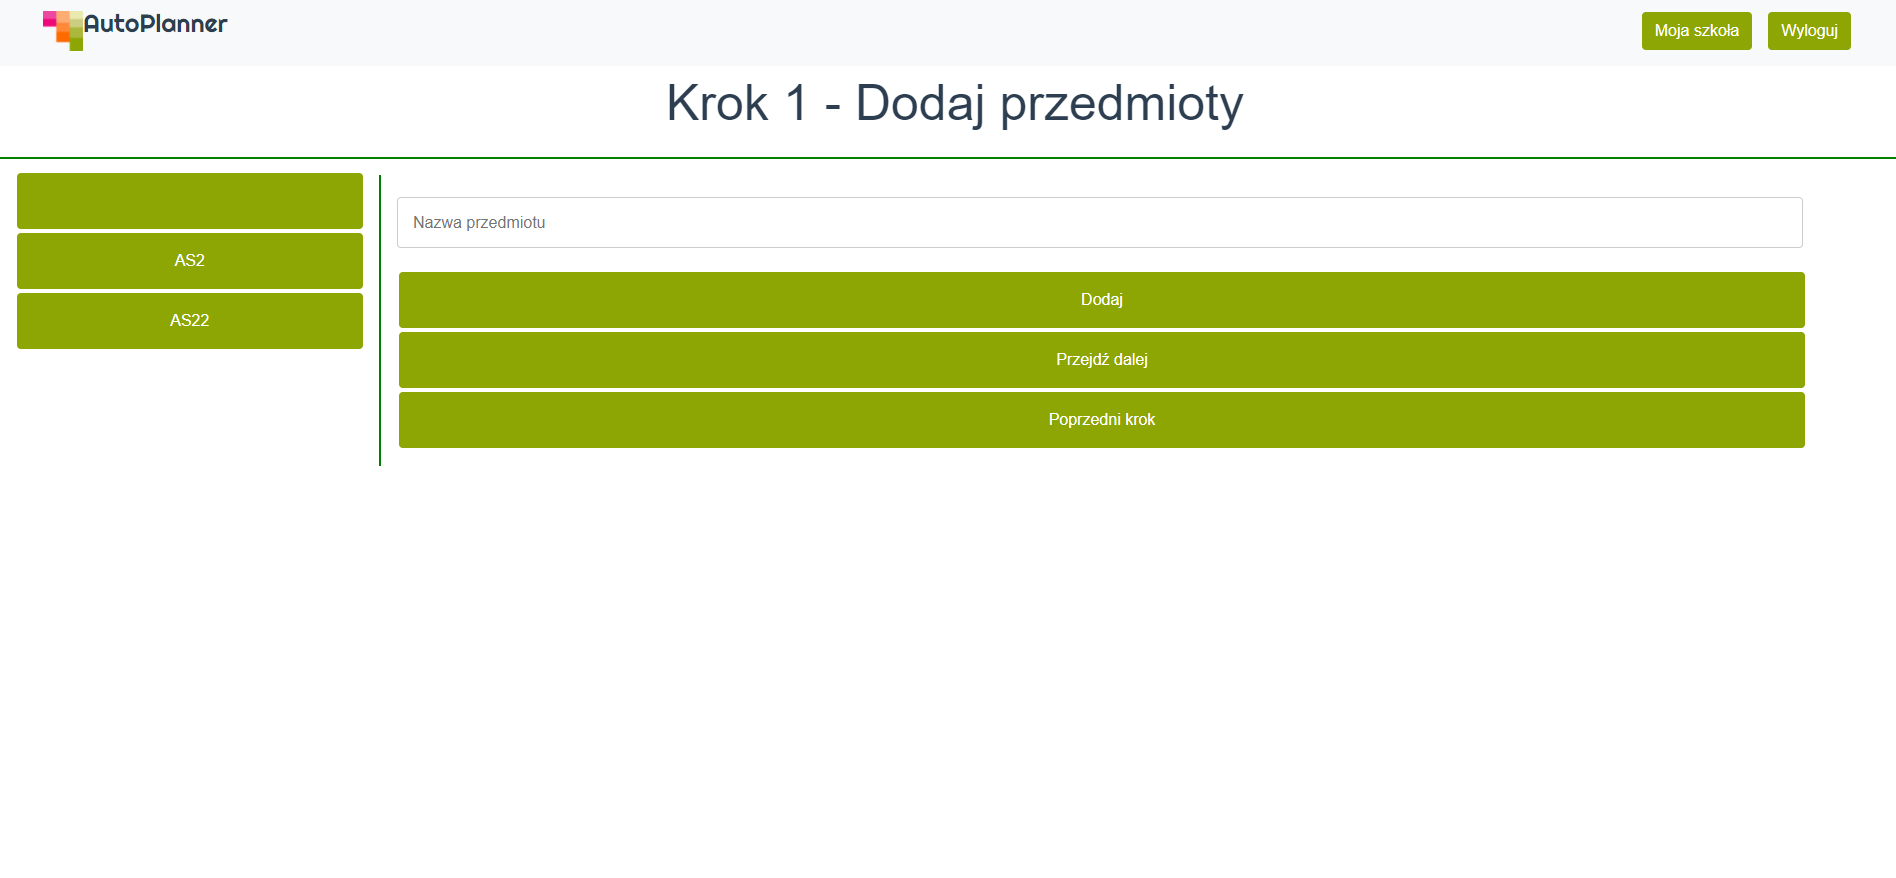
\includegraphics[width=\textwidth]{figures/subject}
\caption{Aplikacja internetowa - Widok dodawania przedmiotów}\label{rys:subject}
\end{figure}
\subsection{Dodawanie nauczycieli}
\begin{figure}[t]
\centering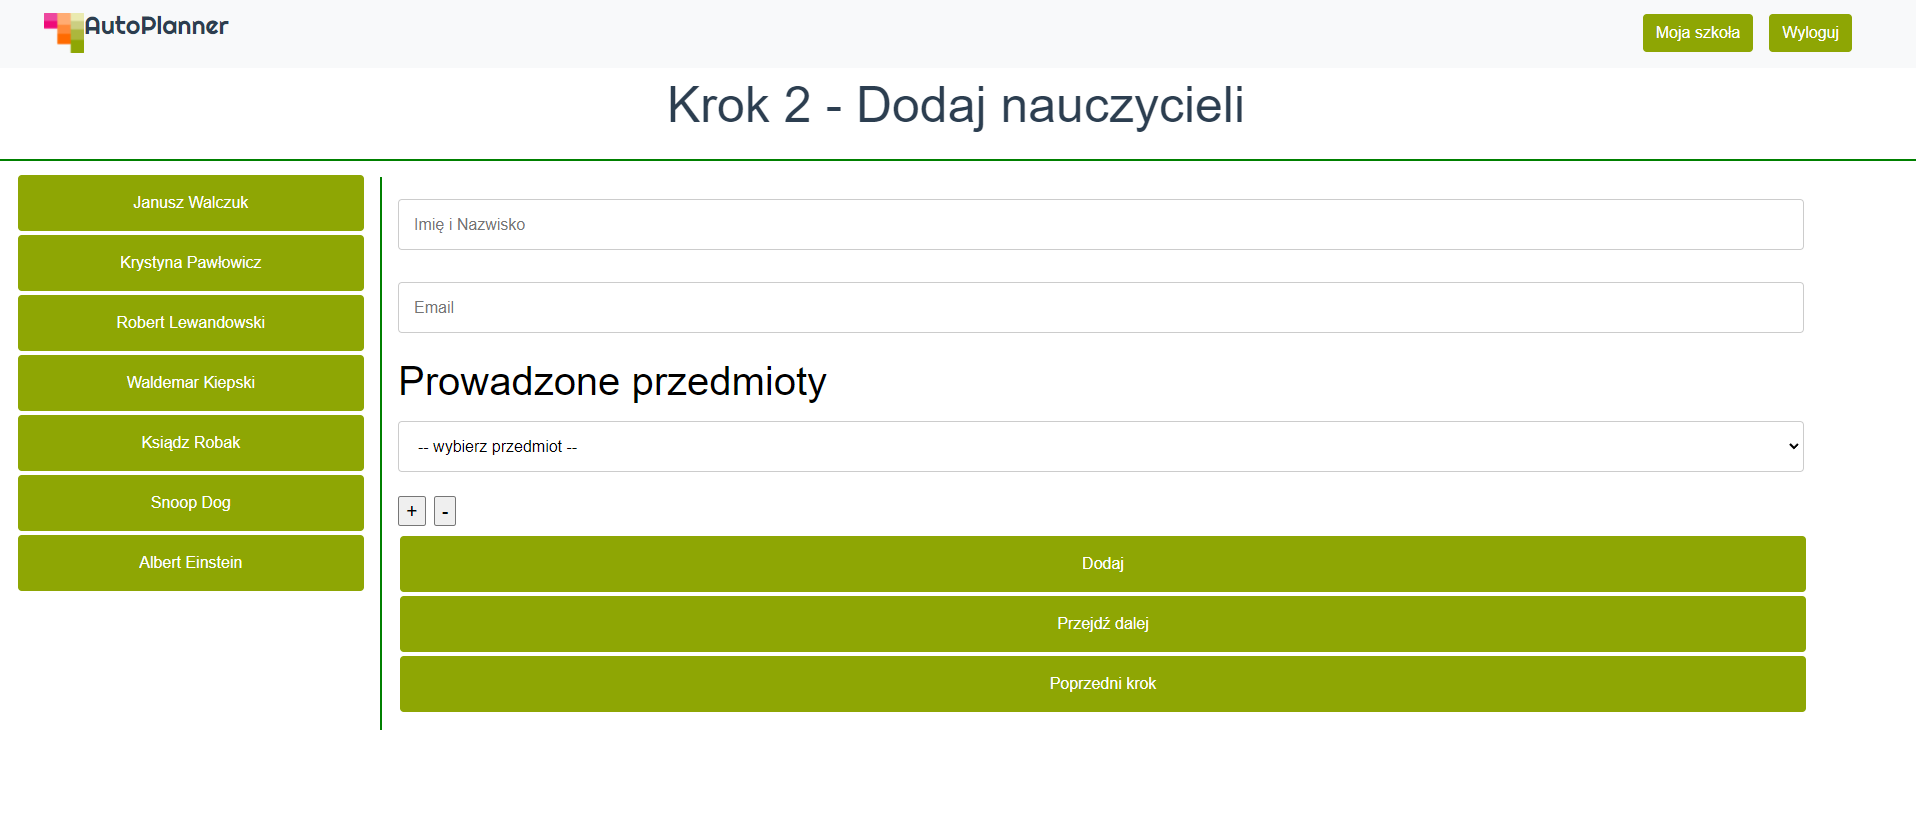
\includegraphics[width=\textwidth]{figures/teacher}
\caption{Aplikacja internetowa - Widok dodawania nauczycieli}\label{rys:teacher}
\end{figure}
\subsection{Dodawanie sali lekcyjnych}
\begin{figure}[t]
\centering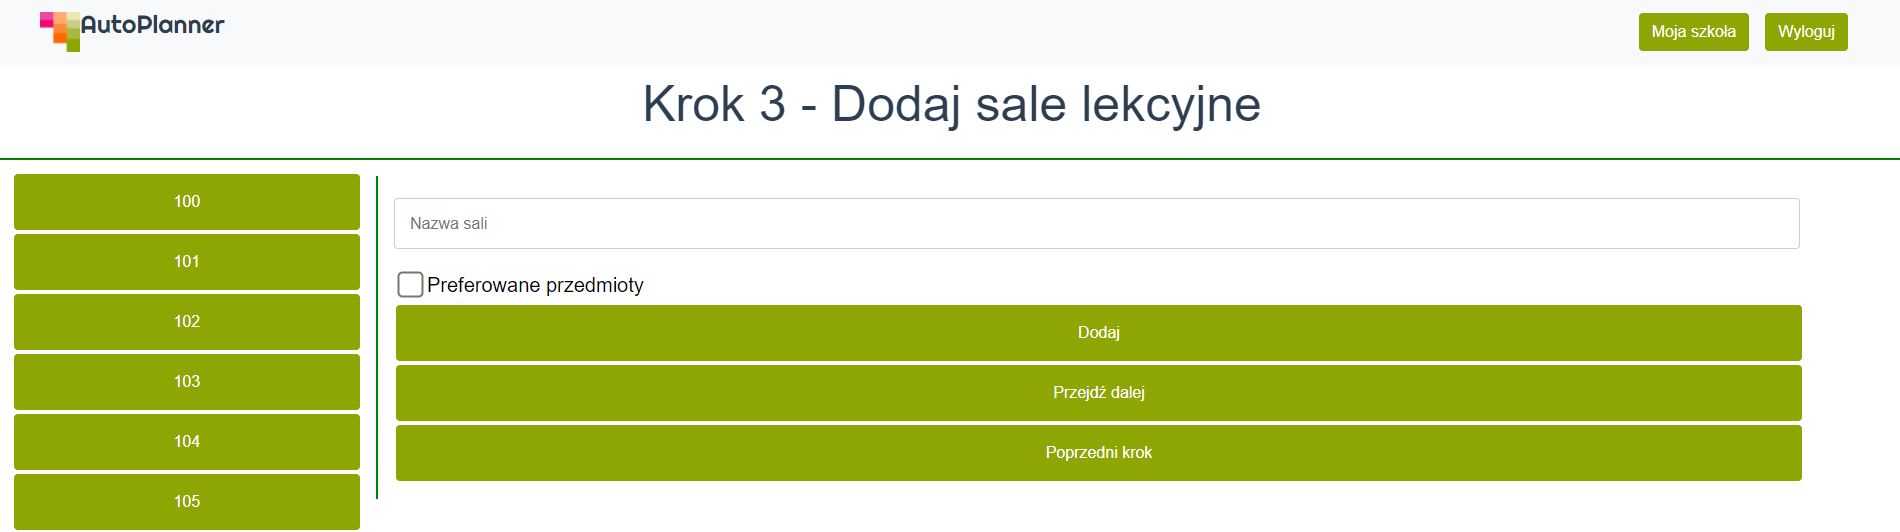
\includegraphics[width=\textwidth]{figures/classroom}
\caption{Aplikacja internetowa - Widok dodawania sali lekcyjnych}\label{rys:classroom}
\end{figure}
\subsection{Dodawanie klas}
\begin{figure}[t]
\centering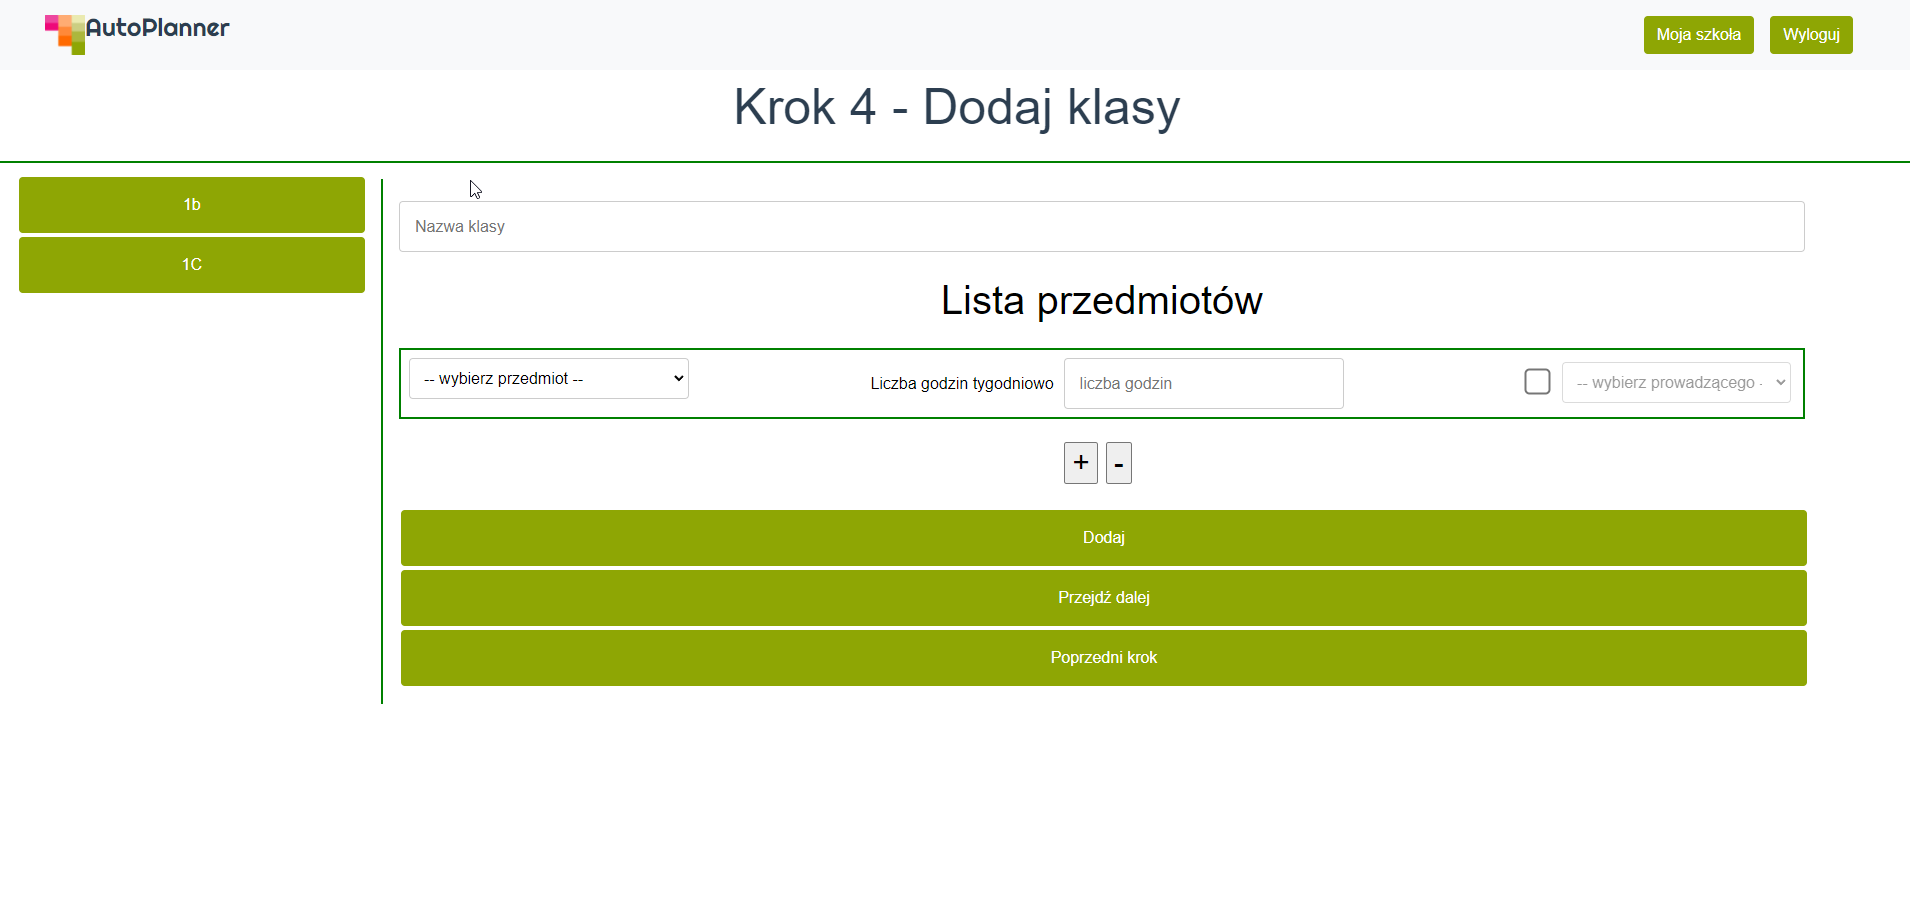
\includegraphics[width=\textwidth]{figures/class}
\caption{Aplikacja internetowa - Widok dodawania klas}\label{rys:class}
\end{figure}
\subsection{Edycja danych}
\begin{figure}[t]
\centering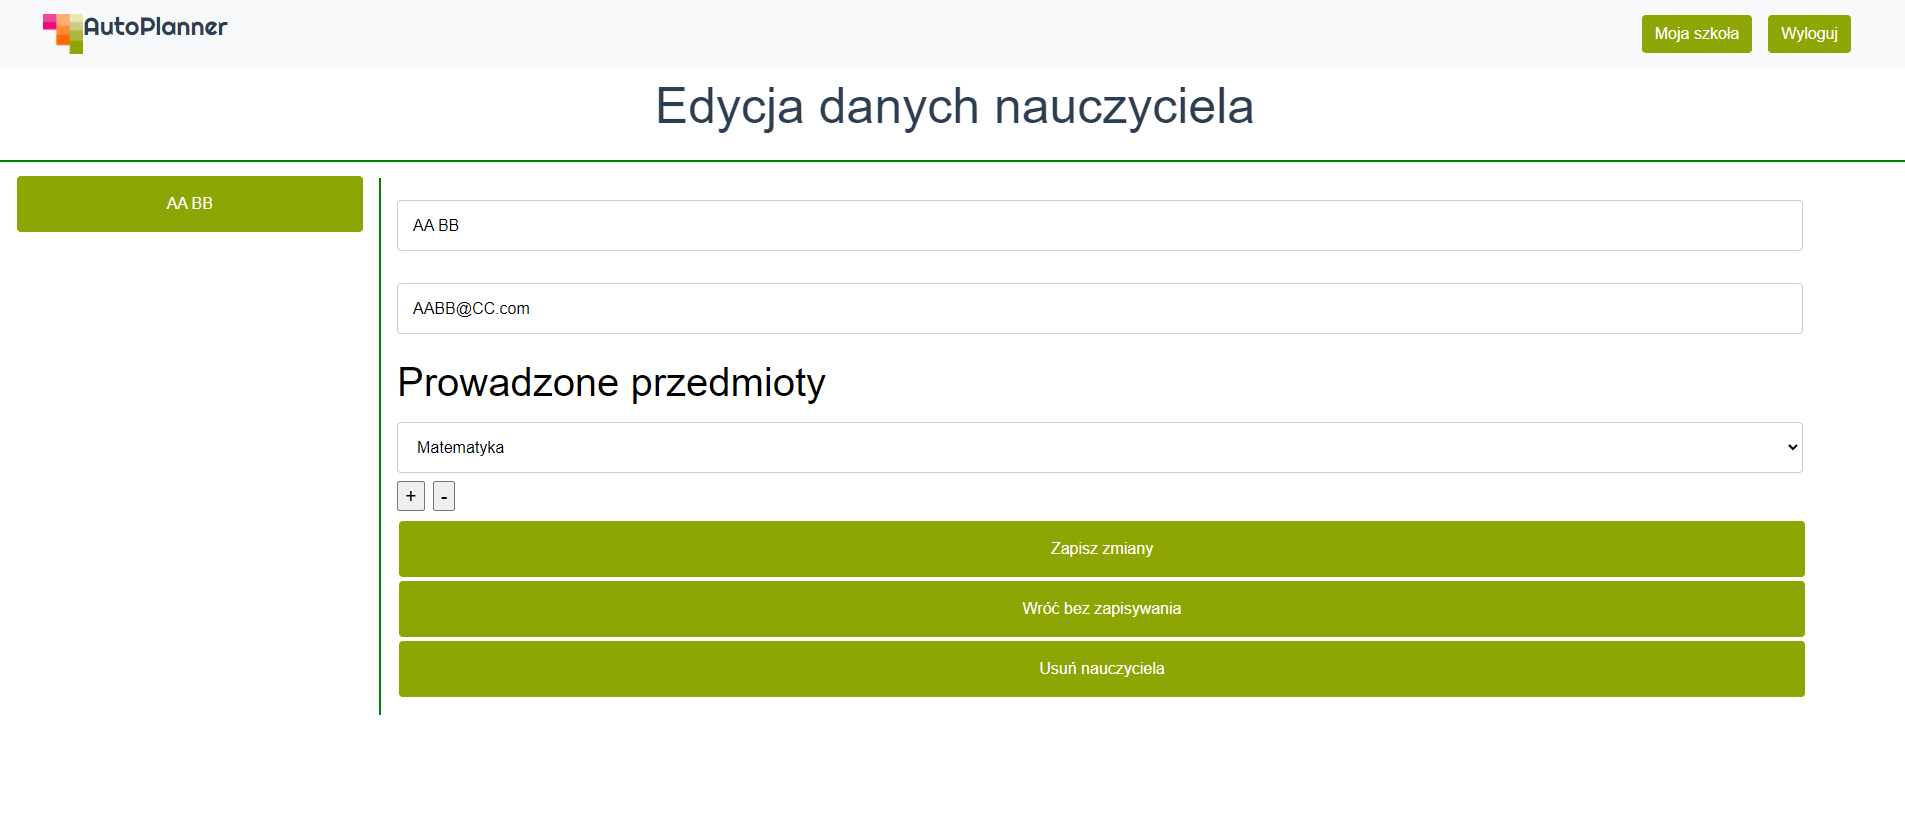
\includegraphics[width=\textwidth]{figures/edit}
\caption{Aplikacja internetowa - Widok edycji danych nauczyciela}\label{rys:edit}
\end{figure}




